\section{Frequenzgang}{114} 

Wird ein Sinus-Signal $u(t)$ in ein LZI-System gegeben, so ist das Ausgangssignal $y(t)$ wieder sinusförmig.
Dabei ändern sich meist die \textbf{Amplitude} und die \textbf{Phase}.
Die \textbf{Frequenz} hingegen bleibt \textbf{gleich}.\\
Die Amplitude und die Frequenz des Ausgangssignals (bzw. deren Änderung) kann allerdings frequenzabhängig sein!

\begin{minipage}[c]{0.48\columnwidth}
    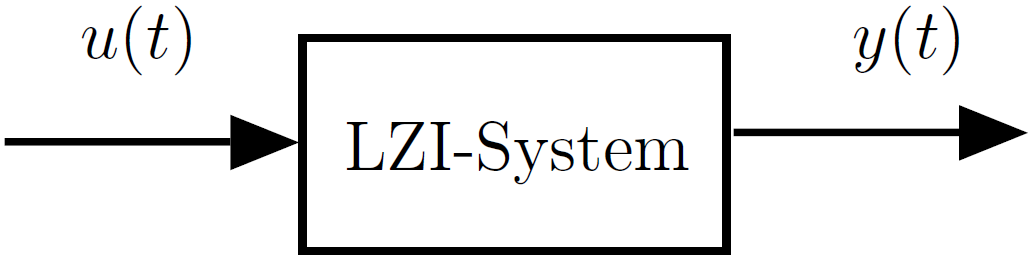
\includegraphics[width=\columnwidth]{images/lzi_system.png}
\end{minipage}
\hfill
\begin{minipage}[c]{0.48\columnwidth}
    \begin{tabular}{ll}
        $A$             & Amplitude Eingangssignal \\
        $B$             & Amplitude Ausgangssignal \\
        $\frac{B}{A}$   & Verstärkung \\
        $\varphi$       & Phasenverschiebung \\
    \end{tabular}
\end{minipage}

\fbox{\parbox{0.8\columnwidth}{
\begin{tabular}{l c l}
    $ u(t) = A \cdot \cos(\omega t) $ & & $ y(t) = B \cdot \cos(\omega t + \varphi) + \text{Transiente} $
\end{tabular}
}}

\subsubsection*{Transiente}

 Die Transiente beschreibt den Vorgang, bis der eingeschwungene Zustand (\textbf{steady state}) erreicht ist.
 In der Praxis betrachtet man häufig $t = 5 \tau$ als Ende des Einschwingvorgangs \\
 \textrightarrow\ \textbf{Uns interessiert nur der der steady state!}


\subsubsection*{Darstellung des Frequenzgangs}

% Der Frequenzgang stellt die Informationen zu einem System im Frequenzbereich dar. Es handelt sich hierbei um dieselben Informationen
% wie im Zeitbereich. Allerdings sind die Berechnungen im Frequenzbereich wesentlich einfacher als im Zeitbereich \\
Der Frequenzgang kann mittels folgenden Diagrammen dargestellt werden: 

\begin{itemize}
    \item Nyquist-Plot (Ortskurve)
    \item Bode-Plot
    \item Zeiger-Diagramm
\end{itemize}


\subsection[Frequenzgang G(j omega) als komplexe Zahl]{Frequenzgang $G(\jimg \omega)$ als komplexe Zahl}{116}

\vspace{-0.3cm} % reduce space 
$$ \boxed{ G(\jimg \omega) =  \abs{G(\jimg \omega)} \cdot \e^{\jimg \angle G(\jimg \omega)} = \frac{B}{A} \cdot \e^{\jimg  \varphi} } $$


\subsection{Frequenzgang der Grundglieder}{117}

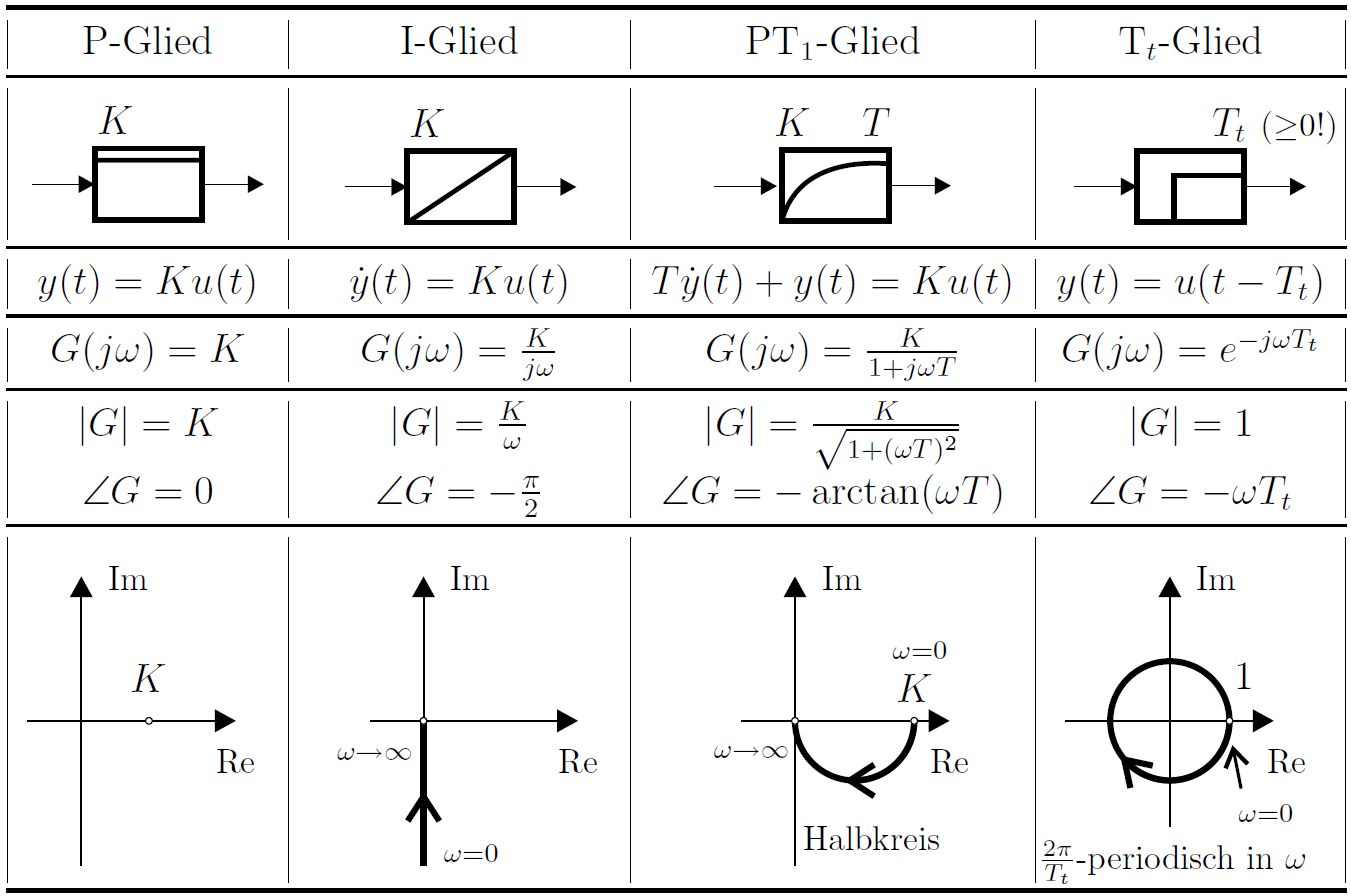
\includegraphics[width=\columnwidth]{images/frequenzgaenge_grundglieder.png} \\
\textrightarrow\ Zusammengesetzte Grundglieder: siehe Skript S. 204-208


\subsection{Darstellung mit Zeigern}{118}

Im Frequenzbereich kann ein Signal \textbf{bei einer bestimmten Frequenz} als Zeigerdiagramm dargestellt werden.
Dabei wird das Signal $\underline{y}(t)$ als Zeiger $\underline{Y}$ zur Zeit $t=0$ dargestellt, welcher anschliessend mit Frequenz $\omega = 2 \pi f$ rotiert.
Das zeitliche Signal $y(t)$ entspricht dem \textbf{Realteil} von $\underline{y}(t)$

\begin{minipage}[c]{0.4\columnwidth}
    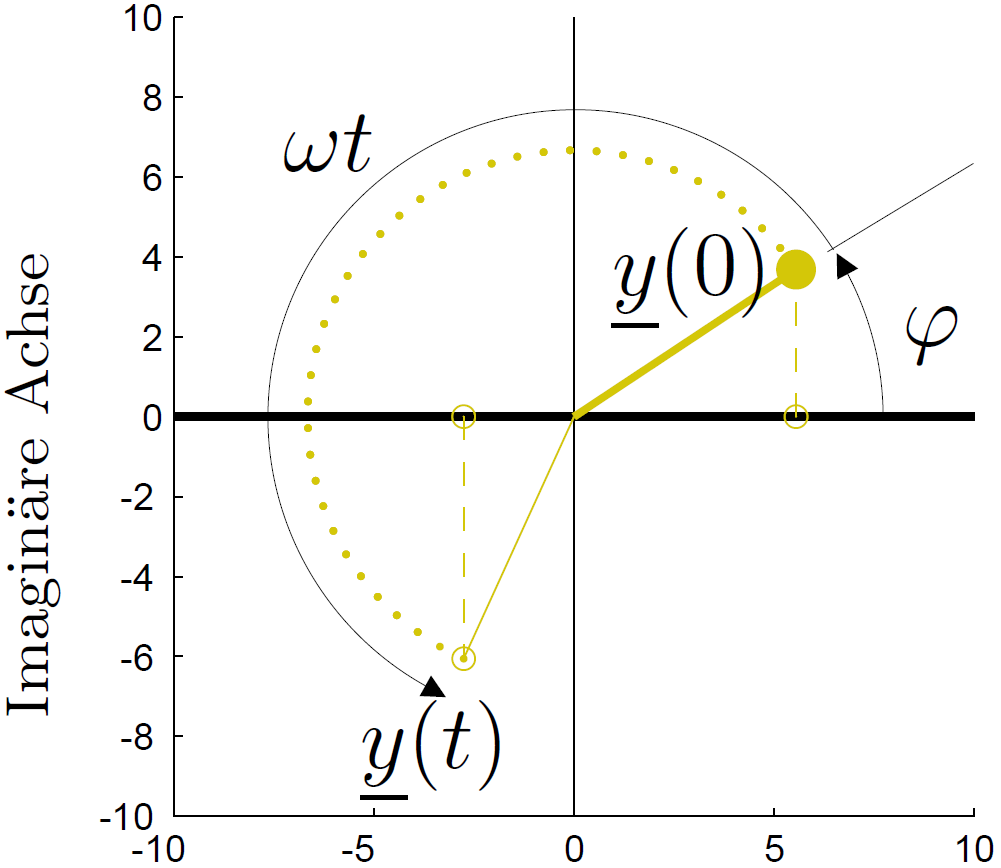
\includegraphics[width=\columnwidth]{images/zeigerdiagramm_1.png}
\end{minipage}
\hfill
\begin{minipage}[c]{0.4\columnwidth}
    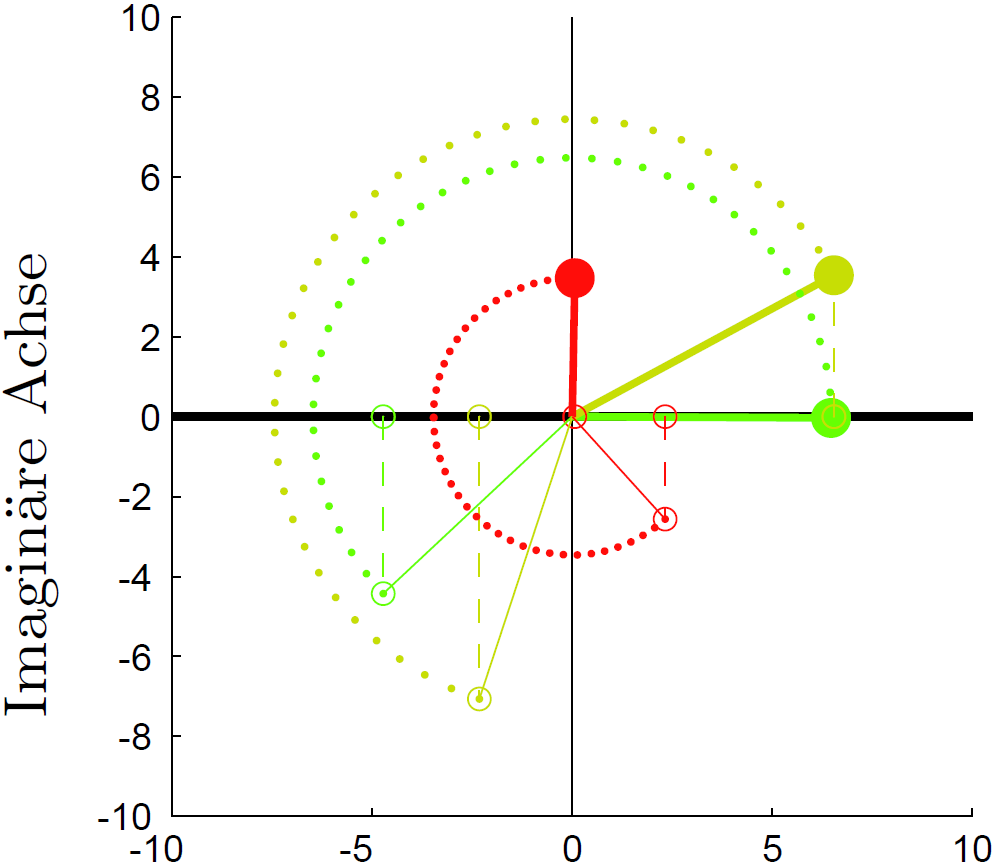
\includegraphics[width=\columnwidth]{images/zeigerdiagramm_2.png}
\end{minipage}


\subsubsection{Komplexe Amplitude $Y$}

\vspace{-0.5cm} % reduce space before align environment
\begin{align*}
    \underline{y}(t) &= B \cdot [\cos(\omega t + \varphi) + \jimg \sin(\omega t + \varphi)] \\
                &= B \cdot e^{\jimg(\omega t + \varphi)} = \cbl{B \cdot e^{\jimg \varphi}} \cdot e^{\jimg \omega t} \\
                &= \cbl{\underline{Y}} \cdot e^{\jimg \omega t}
\end{align*}

Die in der Gleichung vorkommenden Grössen sind definiert als \\
\begin{tabular}{lll}
    $ | \underline{y}(t) | = B$                 & Maximale Amplitude des Ausgangssignals \\
    $ \Re{(\underline{y}(t))} = y(t)$           & Ausgangssignal (zeitlich) \\
    $ \underline{y}(0) = \cbl{\underline{Y}} $  & Anfangszeiger (komplexe Amplitude)
\end{tabular}


\subsubsection{Ableitung / Integral im Frequenzbereich}

\begin{minipage}[c]{0.48\columnwidth}
    $$ \boxed{ \underline{\dot{y}}(t) = \underline{Y} \cdot \jimg \omega \cdot \e^{\jimg \omega t} } $$
\end{minipage}
\hfill
\begin{minipage}[c]{0.48\columnwidth}
    $$\boxed{ \int y(t) \, \diff t = \frac{\underline{Y}}{\jimg \omega} \cdot \e^{\jimg \omega t} } $$
\end{minipage}


\subsection{Bestimmung des Frequenzgangs aus DGL}

\begin{enumerate}
    \item DGL des Systems in Frequenzbereich transformieren
    \item Geeignet umformen: $G(\jimg \omega) = \frac{\underline{Y}}{\underline{U}}$
    \item Falls gewünscht: Amplitude $|G(\jimg \omega)|$ und Phase $\varphi$ bestimmen
\end{enumerate}


\example{$\text{PT}_1$ Glied}

\vspace{-0.3cm} % reduce space
$$ T \dot{y} + y(t) = K u(t) \quad \underrightarrow{\text{Frequenzbereich}} \quad 
T \cdot \jimg \omega \cdot \underline{Y} + \underline{Y} = [\jimg \omega T + 1] \cdot \underline{Y} = K \underline{U} $$
$$ \frac{\underline{Y}}{\underline{U}} = \frac{K}{\jimg \omega T + 1} = G(\jimg \omega) $$
$$ |G(\jimg \omega)| = \frac{|\underline{Y}|}{|\underline{U}|} = \frac{K}{\sqrt{(\omega T)^2 + 1^2}} \qquad \varphi = \arctan \left\lgroup \frac{\Im{G(\jimg \omega)}}{\Re{G(\jimg \omega)}}\right\rgroup + \pi$$


\subsubsection{Allgemeiner Fall}{120}


\vspace{-0.5cm} % reduce space before align environment
\begin{align*}
    a_n y(t)^{(n)} + \cdots  + a_1 \dot{y}(t) + a_0 y(t) &= b_m u(t)^{(m)} + \cdots + b_1 \dot{u}(t) + b_0 u(t) \\
    a_n (\jimg \omega)^n \cdot \underline{Y} + \cdots + a_1 \jimg \omega \cdot \underline{Y} + a_0 \underline{Y} 
    &=  b_m (\jimg \omega)^m \cdot \underline{U} + \cdots + b_1 \jimg \omega \cdot \underline{U} + b_0 \underline{U} \\
    \frac{\underline{Y}}{\underline{U}} 
    &= \frac{b_m (\jimg \omega)^m + \cdots + b_1 \jimg \omega + b_0}{a_n (\jimg \omega)^n + \cdots + a_1 \jimg \omega + a_0} = G(\jimg \omega) \\
    |G(\jimg \omega)| = \frac{|\underline{Y}|}{|\underline{U}|}
    &= \frac{| b_m (\jimg \omega)^m + \cdots + b_1 \jimg \omega + b_0 |}{| a_n (\jimg \omega)^n + \cdots + a_1 \jimg \omega + a_0 |} \\
    \varphi = \angle G(\jimg \omega) &= \arctan \left\lgroup \frac{\Im{G(\jimg \omega)}}{\Re{G(\jimg \omega)}}\right\rgroup (+ \pi)
\end{align*}


\subsection{Serieschaltung von LZI-Systemen}{121}

\begin{center}
    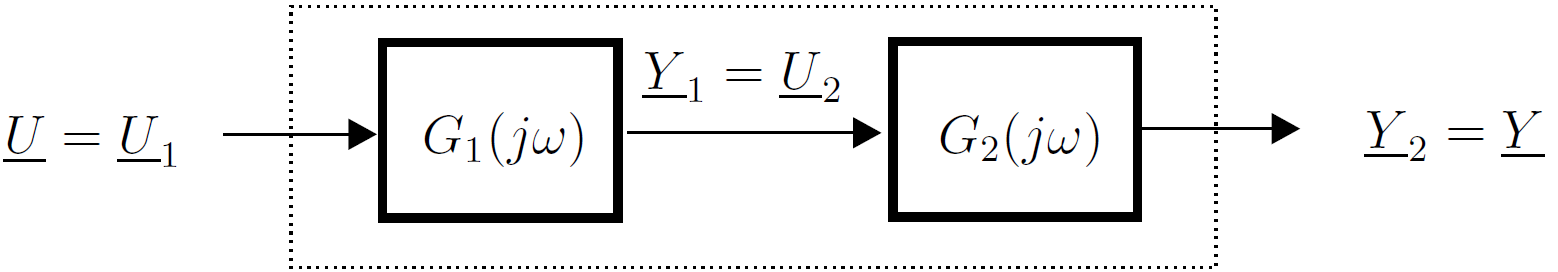
\includegraphics[width=0.7\columnwidth]{images/frequenzgang_serieschaltung.png}
\end{center}
$$ \boxed{ \underline{Y} = \underbrace{G_1(\jimg \omega) \cdot G_2(\jimg \omega)}_{G(\jimg \omega)} \cdot \underline{U} } $$
$$ G_1 \cdot G_2 = |G_1| \cdot \e^{\jimg \angle G_1} \cdot |G_2| \cdot \e^{\jimg \angle G_2} = |G_1| |G_2| \cdot \e^{\jimg (\angle G_1 + \angle G_2)} $$


\subsection{Parallelschaltung von LZI-Systemen}{124}

\begin{center}
    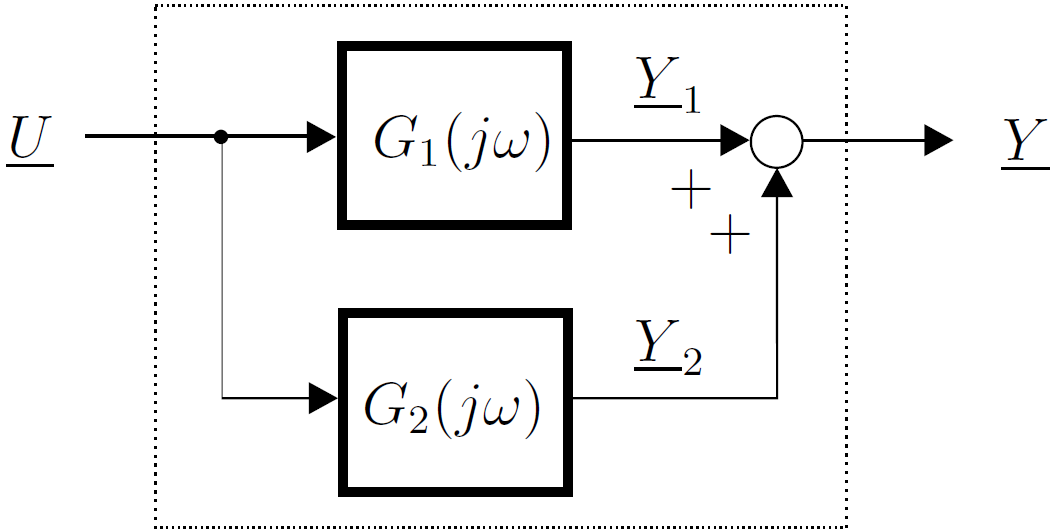
\includegraphics[width=0.5\columnwidth]{images/frequenzgang_parallelschaltung.png}
\end{center}
$$ \boxed{ \underline{Y} = \underline{Y}_1 + \underline{Y}_2 = G_1(\jimg \omega) \cdot \underline{U} + G_2(\jimg \omega) \cdot \underline{U} 
    = \underbrace{(G_1(\jimg \omega) + G_2(\jimg \omega))}_{G(\jimg \omega)} \cdot \underline{U}} $$
$$ G_1 + G_2 = \mathrm{Re}\{ G_1 \} + \mathrm{Re}\{ G_2 \} + \jimg ( \mathrm{Im}\{ G_1 \} + \mathrm{Im}\{ G_2 \}) $$


\subsection{Kreisschaltung (Gegenkopplung) von LZI-Systemen}{124-125}

\begin{minipage}[c]{0.5\columnwidth}
    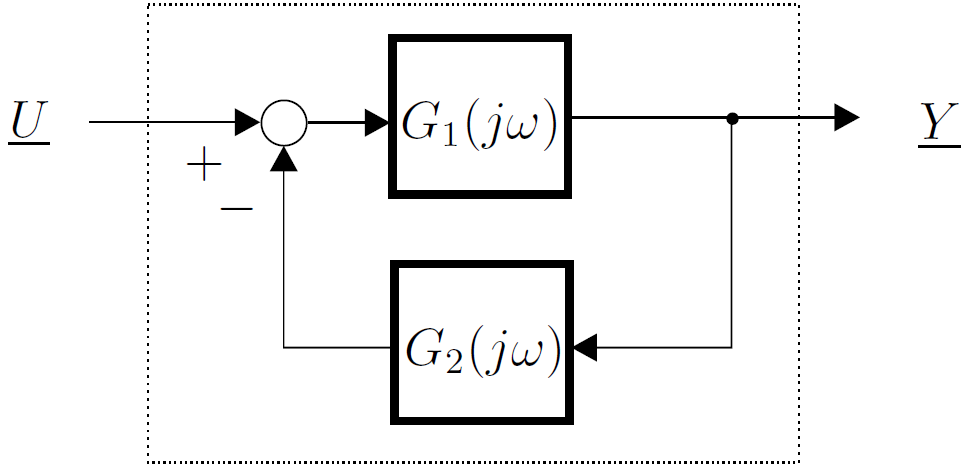
\includegraphics[width=\columnwidth]{images/frequenzgang_kreisschaltung.png}
\end{minipage}
\hfill
\begin{minipage}[c]{0.48\columnwidth}
    $$ \boxed{ \underline{Y} = \underbrace{\frac{G_1(\jimg \omega)}{1 + G_1(\jimg \omega) \cdot G_2(\jimg \omega)}}_{G(\jimg \omega)} \cdot \underline{U}} $$
    \textrightarrow\ Anwendung von \textbf{Mason's Regel}
\end{minipage}


\subsubsection{Vorgehen Frequenzgang ermitteln}
\begin{enumerate}
    \item Gleichung zum Blockdiagramm aufstellen
    \item Nach $\underline{Y}$ umformen 
\end{enumerate}

\subsection{Frequenzgang -- Übertragungsfunktion (UTF)}

Der Frequenzgang $G(\jimg \omega)$ und du Übertragungsfunktion $G(s)$ mit $s = \sigma + \jimg \omega$ hängen folgendermassen zusammen:
$$ \boxed{G(\jimg \omega) = G(s) \big\vert_{s = \jimg \omega}} $$

\subsubsection{Übersicht Darstellungsformen}

\begin{center}
    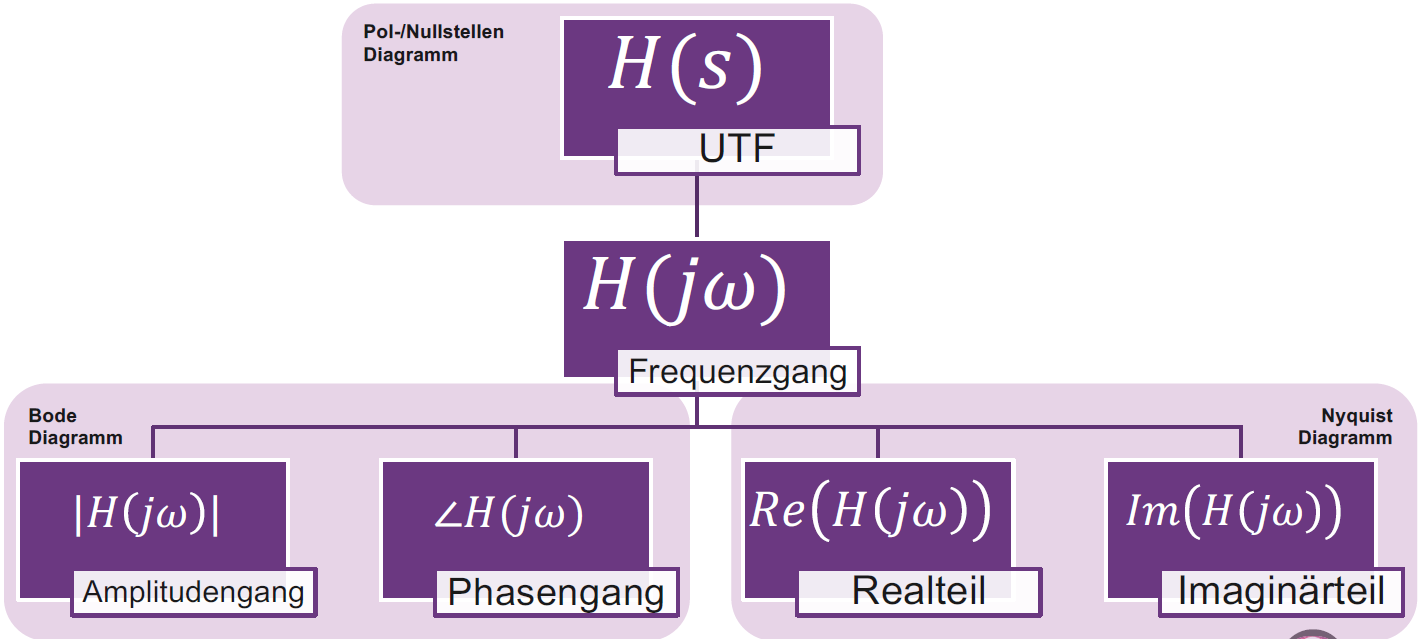
\includegraphics[width=0.75\columnwidth]{images/darstellungen_frequenzgang_utf.png}
\end{center}

